\documentclass{article}
\usepackage{graphicx}
\usepackage{adjustbox}
\usepackage{blindtext}
\usepackage{float}
\pdfminorversion=5 
\pdfcompresslevel=9
\pdfobjcompresslevel=3
\begin{document}

\title{Design Document}
\author{Boriero Stefano  876106  
Brunitti Simone   875039 }


\maketitle

\tableofcontents

\section{Introduction}
\subsection{Purpose}
The purpose of this document is to present the architectural structure of the system that is going to be developed. First an overview of high level components is going to be provided, then more detailed views are going to descibe the low level interaction between thi components. Runtime views will describe how this interaction take place in real time situation. A brief summary of the architectural styles and decisions that have been made will end the first part of the document, followed by the design of the main algorithms.  
User interface is presented using both a formal notation with UX diagrams and visual mock-ups.  
Requirements traceability will close the document explaining how the requirements highlited in the RASD are going to be fulfilled by the designed architecture. 
\subsection{Scope}
Our design architecture will focus mostly on the server side of the system, as we try to keep the client as thin as possible. The part of the system that will run on the car will be analysed as well, as the interaction between the server and the car will define business logic boundaries.
\subsection{Glossary}
\begin{table}[H]
\centering
\caption{Glossary}
\label{my-label}
\begin{tabular}{|l|p{8cm}|}
\hline

TERM & MEANING\\
\hline


API & Application Programming Interface\\\hline
REST &  Representational state transfer: an architectural style providing interoperability between computer systems on the Internet  \\ \hline
UX & Diagrams User experience diagrams  \\ \hline
Payment Gateway & Service that alllows the user to pay through the Internet \\ \hline
Push Notification & A system to notify the user of some changes \\ \hline
DB & Database\\ \hline
Google Maps & A map service offered by Google \\ \hline
Exception & A programming method used to deal with errors \\ \hline
JEE & Java Enterprise Edition \\ \hline
JPA & Java Persistence API \\ \hline
\end{tabular}
\end{table}
\subsection{Reference Document}
-http://www.w3schools.com/graphics/google-maps-intro.asp For references on Google Maps API  \\
-MyTaxiService Design Document Sample \\
-Our PowerEnJoy RASD https://github.com/StefanoBoriero/PowerEnjoy-Boriero-Brunitti/blob/master/releases/RASD-v1.md
\newpage
\section{Architectural design}
\subsection{Overview}
\begin{figure}[ht]
  \begin{adjustbox}{addcode={\begin{minipage}{\width}}{\caption{%
     Overview of the system
      }\end{minipage}},rotate=0,center}
      \includegraphics[width=5in]{"DesignDocument/HighLevel".jpg}%
  \end{adjustbox}
\end{figure}

Both client's and employee's application will communicate with the WebServer throught an HTTP channel, using a Web Browser.
The WebServer will translate Http requests into API method call on the API Server, that will interact with the DataBase Server.
The on-board Car Application will communicate directly with API Server throught a TCP-IP channel to have better performance
while monitoring the real-time ride.
\newpage
\subsection{Component view}

\begin{figure}[ht]
  \begin{adjustbox}{addcode={\begin{minipage}{\width}}{\caption{%
      Middle level component view
      }\end{minipage}},rotate=90,center}
      \includegraphics[width=5.7in]{"DesignDocument/MiddleLevelComponentView".jpg}%
  \end{adjustbox}
\end{figure} 
\newpage
\begin{figure}[ht]
  \begin{adjustbox}{addcode={\begin{minipage}{\width}}{\caption{%
      Component View
      }\end{minipage}},rotate=90,center}
      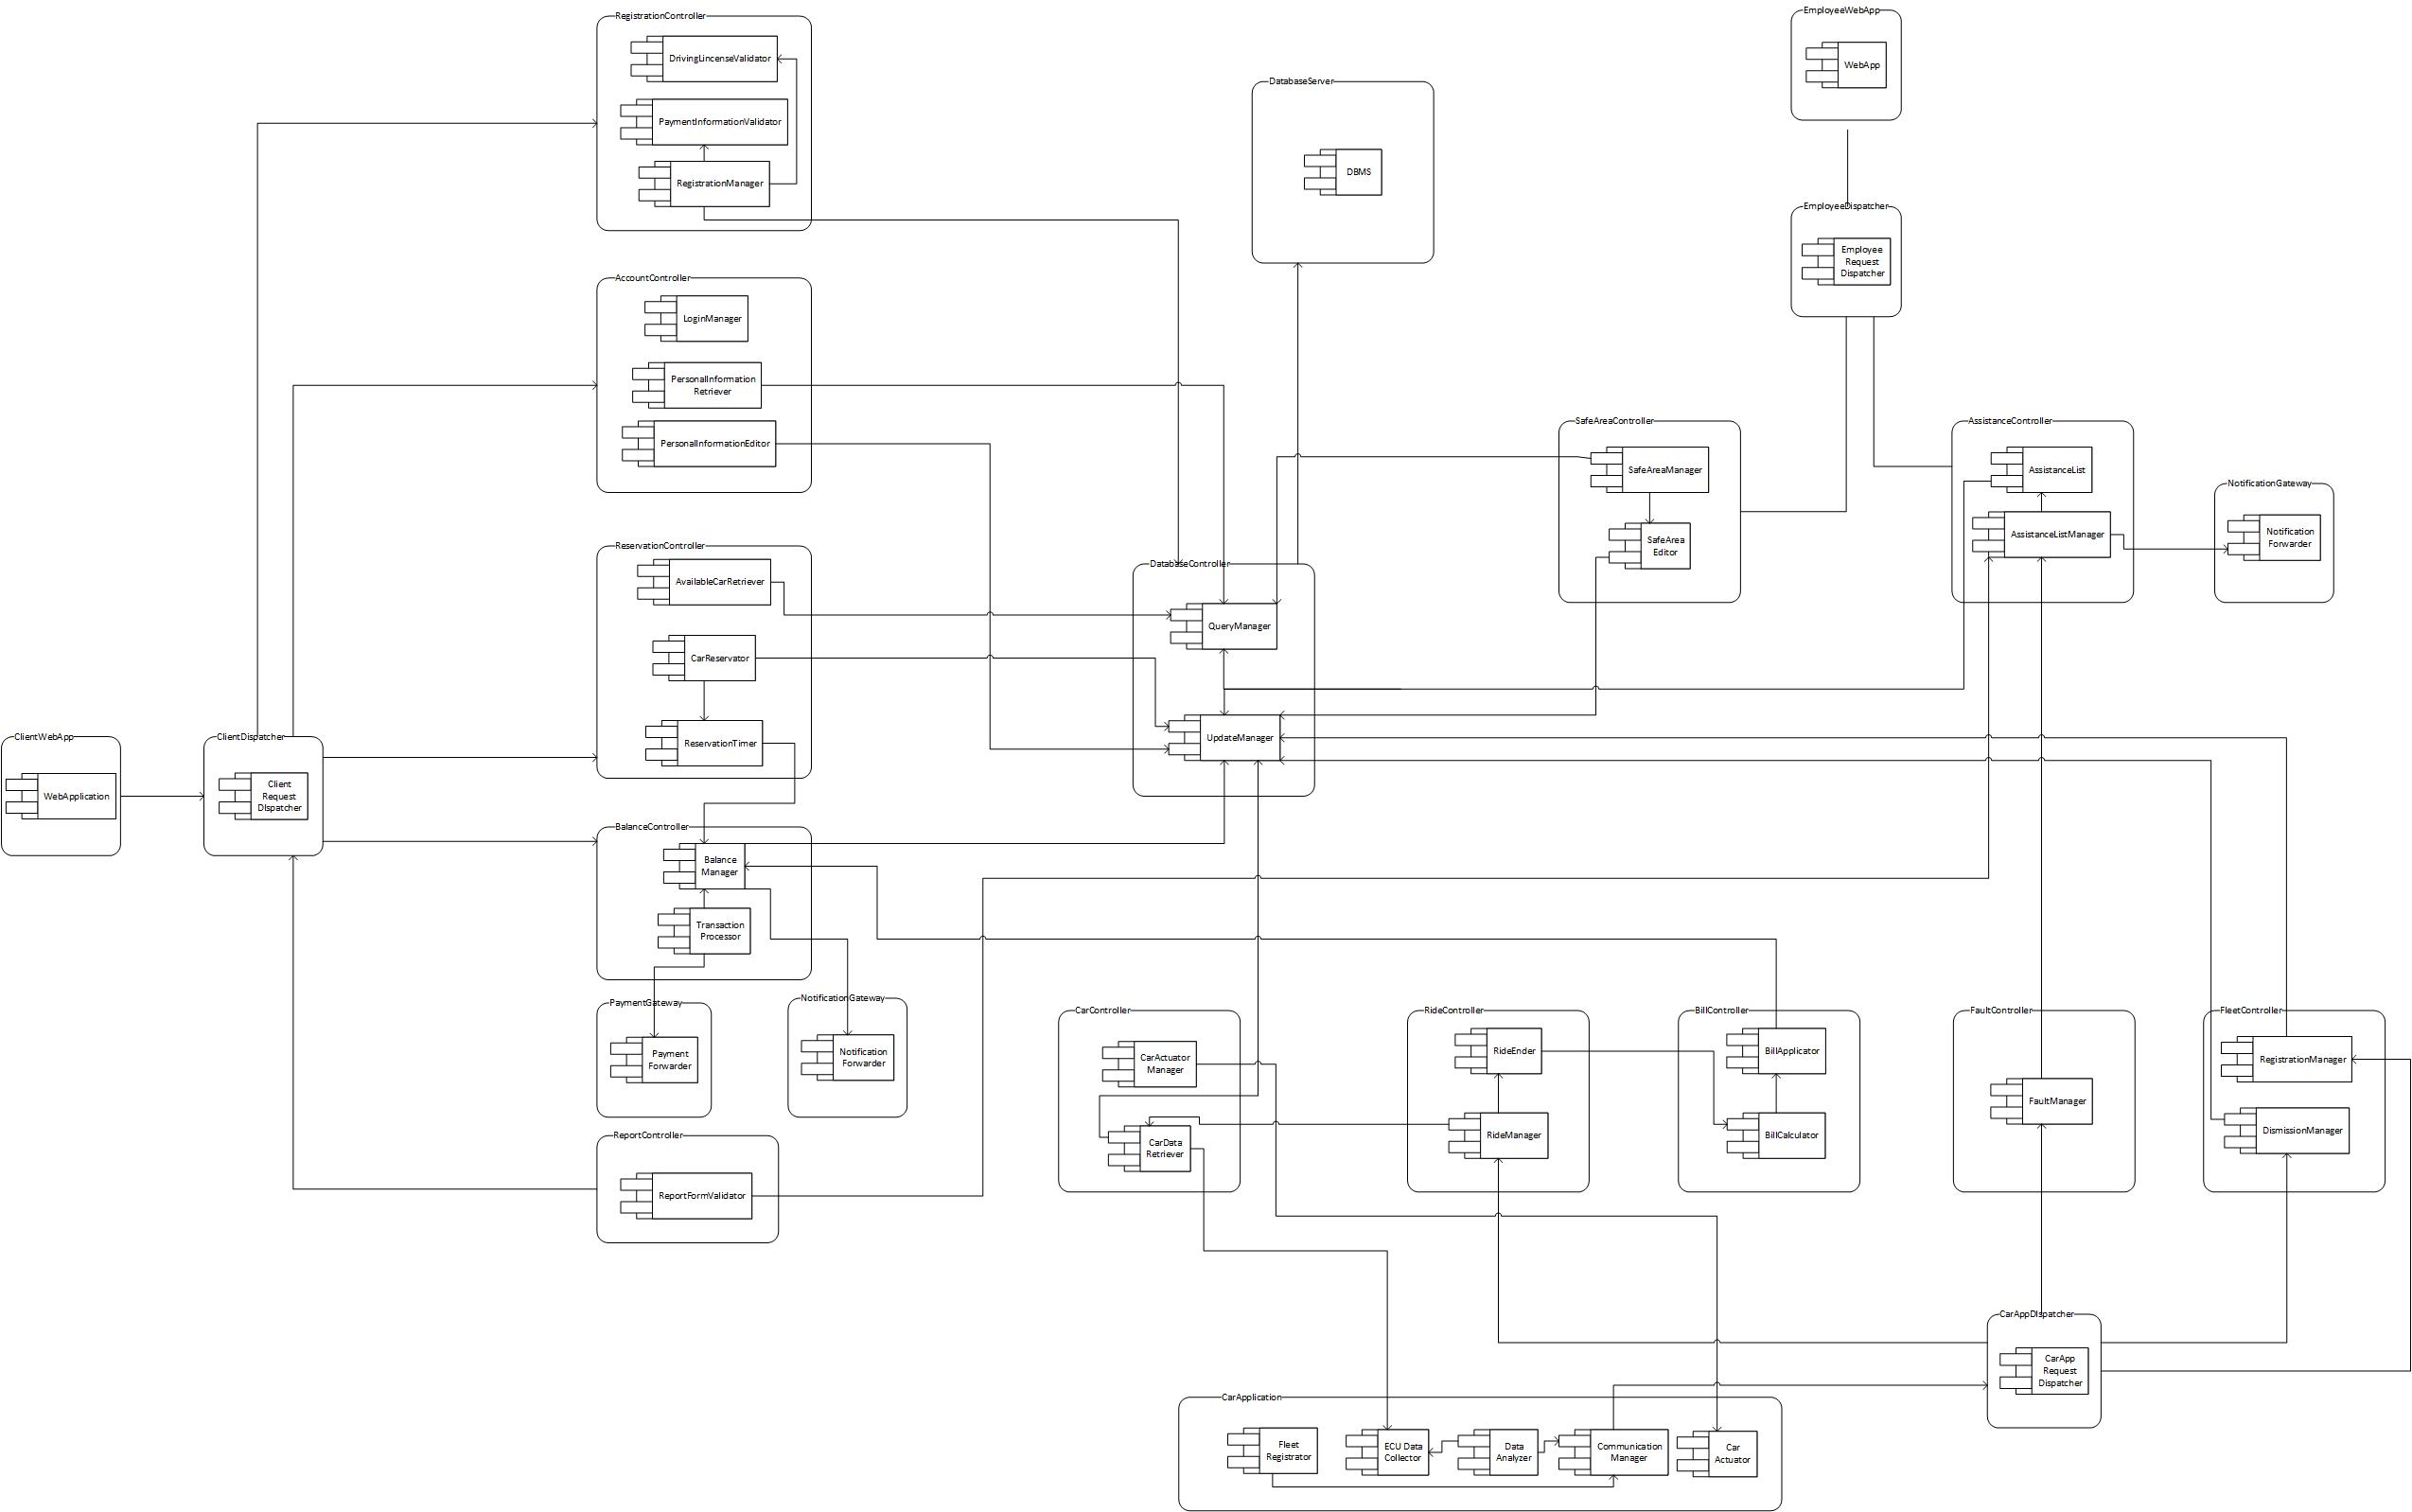
\includegraphics[width=5.9in]{DesignDocument/Components/Images/ComponentView.jpg}%
  \end{adjustbox}
\end{figure}

 

 \newpage
\subsection{Deployment view}
\begin{figure}[ht]
  \begin{adjustbox}{addcode={\begin{minipage}{\width}}{\caption{%
      Deployment view
      }\end{minipage}},rotate=90,center}
      \includegraphics[width=5.5in]{"DesignDocument/Deployment/DeploymentView".jpg}%
  \end{adjustbox}
\end{figure}
\newpage
\subsection{Runtime view}
\subsubsection{Sequence diagrams}


\begin{figure}[ht]
  \begin{adjustbox}{addcode={\begin{minipage}{\width}}{\caption{%
      Customer Login
      }\end{minipage}},rotate=90,center}
      \includegraphics[width=5.7in]{"DesignDocument/SequenceDiagrams/login sequence diagram alternative version".jpg}%
  \end{adjustbox}
\end{figure}
When the user inputs his login credentials in the application, the application must compare this information with the one contained in the database. To do so, the application sends a request to the Client Dispatcher, which transfers the request to the Account Controller. The Account Controller queries the database to retrieve the password corresponding to the input username and subsequently compares the two passwords. If the comparison is positive, the account controller retrieves the user status and sends it to the application. Finallly, the application shows the client a different screen depending on the user status (if the client is a debtor he can't reserve, so that button will be disabled).
\newpage
\begin{figure}[ht]
  \begin{adjustbox}{addcode={\begin{minipage}{\width}}{\caption{%
      Customer reservation
      }\end{minipage}},rotate=90,center}
      \includegraphics[width=5.5in]{"DesignDocument/SequenceDiagrams/Client_reservation_sequence".jpg}%
  \end{adjustbox}
\end{figure}

When the client selects to navigate to the reservation page from the menu, the app will ask the client to select a search position and a search radius. When the client picks a position, the app will contact the Reservation Controller running on the server by means of the Client Dispatcher. The reservation Controller will then query the DB in order to obtain all the positions of the vehicles which are in the selcted search area. This information is passed to the client app, which uses it to create a map using Google Maps API. Finally, when the user selects a vehicle, a reservation request is sent to the Reservation Controller that will create a new reservation and will change the vehicle status to reserved (starting a 1 hour timer if the reservartion is successfull). Finallly, the client app will show a message indicating the outcome of the operation.
\newpage
\begin{figure}[ht]
  \begin{adjustbox}{addcode={\begin{minipage}{\width}}{\caption{%
      Unlock car
      }\end{minipage}},rotate=90,center}
      \includegraphics[width=5.5in]{"DesignDocument/SequenceDiagrams/Unlock_car_sequence_diagram".jpg}%
  \end{adjustbox}
\end{figure}

When the client selects to navigate to the unlock car page, the Client Application will display a page containing an «unlock car» button. If the user presses this button, the client will get the current device position and send a request to unlock the reserved car to the Car Controller using the Client Dispatcher. When the Car Controller receives this request, it will query the DB to ask for the car that has been reserved by that particular user (if a reservation exists). If a reservation has been made, the Car Controller will compare the two sets of coordinates and check if the car can be unlocked. If this is the case, the Car Controller will update the status off the car in the DB and wiil finally unlock the car, sending a message to the Car Application. Finally, the Client Application will display a message outlining the outcome of the operation.

\newpage
\begin{figure}[ht]
  \begin{adjustbox}{addcode={\begin{minipage}{\width}}{\caption{%
      End of the ride
      }\end{minipage}},rotate=90,center}
      \includegraphics[width=5.5in]{"DesignDocument/SequenceDiagrams/endRideSequence".jpg}%
  \end{adjustbox}
\end{figure}

When engine stops, the on-board car application sends a notification to the server throught the CarAppDispatcher. The RideController will collect all the information regarding the ride using the CarController. If the ride has actually ended (i.e. the car has been parked in a safe area or has been abandoned) the RideController will delegate the calculation of the bill to BillController. When the BillController receives the request, it will calculate the import of the bill according ti company policy, check if any discount is applicable than delegate the payment to BalanceController. This component will query the database to get user's current balance and update it. If after the update the balance is negative, user's status is updated to debtor and a notification is sent to her.
\newpage

\subsubsection{State diagrams}
\begin{figure}[ht]
  \begin{adjustbox}{addcode={\begin{minipage}{\width}}{\caption{%
      User status
      }\end{minipage}},rotate=0,center}
      \includegraphics[width=5.5in]{"DesignDocument/StateDiagrams/UserStateDiagram".jpg}%
  \end{adjustbox}
\end{figure}
\newpage
\subsection{Component interfaces}


\textbf{Registration Controller}\\
\begin{figure}[ht]
  \begin{adjustbox}{addcode={\begin{minipage}{\width}}{\caption{%
      Registration Controller
      }\end{minipage}},rotate=0,center}
      \includegraphics[width=4in]{"DesignDocument/Components/Images/RegistrationController".jpg}%
  \end{adjustbox}
\end{figure}\\
\textbf{INTERFACE}: 
 \newline
-\textbf{register(personal-info)} checks if the informations are valid, then the user is added to the database  
\newline
-\textbf{InvalidInformationException} this exception is raised if the 	information are incorrect  
\newline
\textbf{USES}:   
\newline
-\textbf{databaseController}
\newpage
\textbf{Account Controller}\\
\begin{figure}[ht]
  \begin{adjustbox}{addcode={\begin{minipage}{\width}}{\caption{%
      Account Controller
      }\end{minipage}},rotate=0,center}
      \includegraphics[width=4in]{"DesignDocument/Components/Images/AccountController".jpg}%
  \end{adjustbox}
\end{figure}\\
\textbf{INTERFACE}: 
 \newline
-\textbf{login():} enables users to log in   
\newline
-\textbf{get-personal-info():} gets user's personal information from the database 
\newline
-\textbf{edit-personal-info():} updates user's personal information in the database \\
-\textbf{signal-infraction(infraction-info):} changes user's status to signalled in the database  
\newline
\textbf{USES}:   
\newline
-\textbf{databaseController}
\newpage
\textbf{Reservation Controller}\\
\begin{figure}[ht]
  \begin{adjustbox}{addcode={\begin{minipage}{\width}}{\caption{%
     Reservation Controller
      }\end{minipage}},rotate=0,center}
      \includegraphics[width=4in]{"DesignDocument/Components/Images/ReservationController".jpg}%
  \end{adjustbox}
\end{figure}\\
\textbf{INTERFACE}: 
 \newline
-\textbf{get-near-vehicles(position-information):} gets from the database the cars available near the selected position 
\newline
-\textbf{create-reservation(user-info):} creates a new reservation in the database; the selected car won't be available anymore
\newline
-\textbf{UnavailableCarException:} this exception is raised if the selected car is no longer available (another user has reserved it while he was looking at the map)  
\newline 
- \textbf{unlock(user-info):} checks if the user is near the car he reserved: if so, interrupts the resertvation timer then delegates the opening to CarController
\\
\textbf{USES}:   
\newline
-\textbf{databaseController}
\newpage
\textbf{Balance Controller}\\
\begin{figure}[ht]
  \begin{adjustbox}{addcode={\begin{minipage}{\width}}{\caption{%
      Balance Controller
      }\end{minipage}},rotate=0,center}
      \includegraphics[width=4in]{"DesignDocument/Components/Images/BalanceController".jpg}%
  \end{adjustbox}
\end{figure}\\
\textbf{INTERFACE}: 
 \newline
-\textbf{deposit(payment-provider, amount, user):} adds to user's balance the indicated amount of money
\newline
-\textbf{TransactionException:} this exception is raised if the transaction fails 
\newline
-\textbf{pay(amount, user):} subtracts the amount of a bill: if the balance becomes negative, a notification is sent to the user
\newline
\textbf{USES}:   
\newline
-\textbf{databaseController}
\\
-\textbf{paymentGateway}
\\
-\textbf{notificationGateway}
\\
\newpage
\textbf{Report Controller}\\
\begin{figure}[ht]
  \begin{adjustbox}{addcode={\begin{minipage}{\width}}{\caption{%
      Report Controller
      }\end{minipage}},rotate=0,center}
      \includegraphics[width=4in]{"DesignDocument/Components/Images/ReportController".jpg}%
  \end{adjustbox}
\end{figure}\\
\textbf{INTERFACE}: 
 \newline
-\textbf{report-damage(report-form):} adds the car which the report is about in the assistance list   
\newline
\textbf{USES}:   
\newline
-\textbf{assistanceController}
\newpage
\textbf{Safe Area Controller}\\
\begin{figure}[ht]
  \begin{adjustbox}{addcode={\begin{minipage}{\width}}{\caption{%
      Safe Area Controller
      }\end{minipage}},rotate=0,center}
      \includegraphics[width=4in]{"DesignDocument/Components/Images/SafeAreaController".jpg}%
  \end{adjustbox}
\end{figure}\\
\textbf{INTERFACE}: 
 \newline
-\textbf{get-safe-areas():} queries the database to get the set of safe areas already defined   
\newline
-\textbf{create-safe-area(boundaries):} updates the database by adding a new safe area
\newline
-\textbf{OverlapException:} this exception is raised if a newly defined safe area overlaps an already defined one
\newline
\textbf{USES}:   
\newline
-\textbf{databaseController}
\newpage
\textbf{Assistance Controller}\\
\begin{figure}[ht]
  \begin{adjustbox}{addcode={\begin{minipage}{\width}}{\caption{%
      Assistance Controller
      }\end{minipage}},rotate=0,center}
      \includegraphics[width=4in]{"DesignDocument/Components/Images/AssistanceController".jpg}%
  \end{adjustbox}
\end{figure}\\
\textbf{INTERFACE}: 
 \newline
-\textbf{add(vehicle-id):} adds the vehicle to the assistance list; it will no longer be available to reservation  
\newline
-\textbf{take-in-charge(vehicle-id, employee-id):} removes the vehicle from the assitance list as an employee will take care of the car
\newline
-\textbf{NotNeedyVehicleException:} this exception is raised if the vehicle specified is not in the list (i.e. some other employee has taken it in charge while he was choosing what to do)
\newline
-\textbf{solved(vehicle-id):} updates the database to set the vehicle as available as the issue was solved
\newline
\textbf{USES}:   
\newline
-\textbf{databaseController}
\newpage
\textbf{Car Controller}\\
\begin{figure}[ht]
  \begin{adjustbox}{addcode={\begin{minipage}{\width}}{\caption{%
      Car Controller
      }\end{minipage}},rotate=0,center}
      \includegraphics[width=4in]{"DesignDocument/Components/Images/CarController".jpg}%
  \end{adjustbox}
\end{figure}\\
\textbf{INTERFACE}: 
 \newline
-\textbf{unlock-car(vehicle-id)}: forwards the unlock command to the car application\\
-\textbf{TooFarException:} this exception is raised if the user is not close to the car 
\newline
-\textbf{CannotUnlockException:} this exception is raised if the opening fails
\newline
-\textbf{get-car-data(data-type):} dialogs with on-board car application to get the specified data, and updates the database
\newline
\textbf{USES}:   
\newline
-\textbf{ECUDataCollector}\\
-\textbf{carActuator}\\
-\textbf{databaseController}
\newpage
\textbf{Ride Controller}\\
\begin{figure}[ht]
  \begin{adjustbox}{addcode={\begin{minipage}{\width}}{\caption{%
      Ride Controller
      }\end{minipage}},rotate=0,center}
      \includegraphics[width=4in]{"DesignDocument/Components/Images/RideController".jpg}%
  \end{adjustbox}
\end{figure}\\
\textbf{INTERFACE}: 
 \newline
-\textbf{start-ride():} starts the monitoring of car during the ride 
\newline
-\textbf{end-ride(ride-info):} ends the ride, checks if any infraction has been committed (if any signal it to AccountController), collects all the data to calculate the bill and forwards them to the dedicated component
\newline
\textbf{USES}:   
\newline
-\textbf{carController}\\
-\textbf{AccountController}\\
-\textbf{billController}
\newpage
\textbf{Bill Controller}\\
\begin{figure}[ht]
  \begin{adjustbox}{addcode={\begin{minipage}{\width}}{\caption{%
      Bill Controller
      }\end{minipage}},rotate=0,center}
      \includegraphics[width=4in]{"DesignDocument/Components/Images/BillController".jpg}%
  \end{adjustbox}
\end{figure}\\
\textbf{INTERFACE}: 
 \newline
-\textbf{calculate-bill(ride-info):} calculates the amount of the bill, than forwards it to the component dedicated to its application  
\newline
\textbf{USES}:   
\newline
-\textbf{balanceController}
\newpage


\textbf{Fault Controller}\\
\begin{figure}[ht]
  \begin{adjustbox}{addcode={\begin{minipage}{\width}}{\caption{%
      Fault Controller
      }\end{minipage}},rotate=0,center}
      \includegraphics[width=4in]{"DesignDocument/Components/Images/FaultController".jpg}%
  \end{adjustbox}
\end{figure}\\
\textbf{INTERFACE}:
 \newline
-\textbf{notify-fault(fault-info):} receives the information regarding some issues detected by on-board application and adds the car to the assistance list   
\newline
\textbf{USES}:   
\newline
-\textbf{assistanceController}
\newpage
\textbf{Fleet Controller}\\
\begin{figure}[ht]
  \begin{adjustbox}{addcode={\begin{minipage}{\width}}{\caption{%
     Fleet Controller
      }\end{minipage}},rotate=0,center}
      \includegraphics[width=4in]{"DesignDocument/Components/Images/FleetController".jpg}%
  \end{adjustbox}
\end{figure}\\
\textbf{INTERFACE}: 
 \newline
-\textbf{register-car(car-info):} adds a new car to the fleet
\newline
-\textbf{AlreadyRegisteredException:} this exception is raised if the car is already registered in the fleet 
\newline
-\textbf{dismiss-car(car-info):} removes a car from the fleet
\newline
\textbf{USES}:   
\newline
-\textbf{databaseController}
\newpage
\textbf{Car Application}\\
\begin{figure}[ht]
  \begin{adjustbox}{addcode={\begin{minipage}{\width}}{\caption{%
      Car Application
      }\end{minipage}},rotate=0,center}
      \includegraphics[width=4in]{"DesignDocument/Components/Images/CarApplication".jpg}%
  \end{adjustbox}
\end{figure}\\
\textbf{INTERFACE}: 
 \newline
-\textbf{get-data(data-type)} gets the required data from the ECU 
\newline
-\textbf{unlock()} unlocks the car via its actuators  
\newline
\textbf{USES}:   
\newline
-\textbf{carAppDispatcher}
\newpage
\textbf{Payment Gateway}\\
\begin{figure}[ht]
  \begin{adjustbox}{addcode={\begin{minipage}{\width}}{\caption{%
      Payment Gateway
      }\end{minipage}},rotate=0,center}
      \includegraphics[width=3in]{"DesignDocument/Components/Images/PaymentGateway".jpg}%
  \end{adjustbox}
\end{figure}\\
\textbf{INTERFACE}: 
 \newline
-\textbf{forward-payment(payment-info)}  forwards the payment request to the selected payment provider after a deposit has been requested 
\newline
\textbf{USES}:   
\newline
-\textbf{externalPaymentProvider}
\newpage
\textbf{Notification Gateway}\\
\begin{figure}[ht]
  \begin{adjustbox}{addcode={\begin{minipage}{\width}}{\caption{%
      Notification Gateway
      }\end{minipage}},rotate=0,center}
      \includegraphics[width=3in]{"DesignDocument/Components/Images/NotificationGateway".jpg}%
  \end{adjustbox}
\end{figure}\\
\textbf{INTERFACE}: 
 \newline
-\textbf{notify(user, info):} notifies the user after a relevant event has occurred  
\newline
\textbf{USES}:   
\newline
-\textbf{none}
\newpage
\textbf{Client Dispatcher}\\
\begin{figure}[ht]
  \begin{adjustbox}{addcode={\begin{minipage}{\width}}{\caption{%
      Client Dispatcher
      }\end{minipage}},rotate=0,center}
      \includegraphics[width=3in]{"DesignDocument/Components/Images/ClientDispatcher".jpg}%
  \end{adjustbox}
\end{figure}\\
\textbf{INTERFACE}: 
 \newline
-\textbf{dispatch-request(request-info):} forwards client's request to the dedicated component 
\newline
\textbf{USES}:   
\newline
-\textbf{registrationController}\\
-\textbf{accountController}\\
-\textbf{reservationController}\\
-\textbf{balanceController}\\
-\textbf{reportController}\\

\newpage
\textbf{Employee Dispatcher}\\
\begin{figure}[ht]
  \begin{adjustbox}{addcode={\begin{minipage}{\width}}{\caption{%
     Employee Dispatcher
      }\end{minipage}},rotate=0,center}
      \includegraphics[width=3in]{"DesignDocument/Components/Images/EmployeeDispatcher".jpg}%
  \end{adjustbox}
\end{figure}\\
\textbf{INTERFACE}: 
 \newline
-\textbf{dispatch-request(request-info):} forwards employee's request to the dedicated component   
\newline
\textbf{USES}:   
\newline
-\textbf{assistanceController}\\
-\textbf{safeAreaController}
\newpage
\textbf{CarApp Dispatcher}\\
\begin{figure}[ht]
  \begin{adjustbox}{addcode={\begin{minipage}{\width}}{\caption{%
     CarApp Dispatcher
      }\end{minipage}},rotate=0,center}
      \includegraphics[width=3in]{"DesignDocument/Components/Images/CarAppDispatcher".jpg}%
  \end{adjustbox}
\end{figure}\\
\textbf{INTERFACE}: 
 \newline
-\textbf{dispatch-request(request-info):}  forwards request of car application to the dedicated component
\newline
\textbf{USES}:   
\newline
-\textbf{faultController}\\
-\textbf{rideController}\\
-\textbf{fleetController}
\newpage

\subsection{Selected architectural styles and patterns}
\subsubsection{General architecture}
The overall architecture we will adopt to develop the PowerEnJoy platform will be a \textbf{three-tier} architecture with distributed logic. Using this architecture, we will be able to decouple the business logic layer from the presentation and the data layers. Our central system (where we can find the data layer and most of the business logic) needs to communicate both with the user and the vehicles. To achieve this communication, we will use:\\
-A \textbf{client-server} architectural style for the communication with the user. In this case, the client is the user device (pc or mobile device). The client side takes care of the presentation logic and will also contain some business logic (mainly the one used to communicate with the Google Maps service). We will however try to keep the client as thin as possible.\\
-An \textbf{event based paradigm} for the communication between the central system and the vehicles. Since the vehicles will need to notify state changes, the central system will register itself as a listener to all the vehicles and will act accordingly to these state changes. Moreover, the car must expose some methods to the central system (such as the one to unlock the car).\\
\subsubsection{Design decisions}
\textbf{JEE}: we will develop the system using JEE to develop a reliable system in a faster time. Security requirements will be more easily fulfilled using consolidated practices, as well as performance ones. The component-based style will also be reflected in the JEE Bean structure.\\
\textbf{Google Maps API}: the user device will interact directly with Google Maps services through Google Maps APIs. This will allow the device to display useful maps used by the user to access PowerEnjoy services.\\
\textbf{Java Persistence API}: we will use JPA for accessing, persisting, and managing our database, since JPA is already implemented in JEE.\\
\subsubsection{Design patterns}
\textbf{Client-server}: as aforementioned in the introduction of this chapter, we will make large use of the Client-Server design pattern, using it in the communication between the user device and the central system. To achieve this, the server will expose some methods (using a REST architecture) that will be used by the client to access the PowerEnJoy platform services.\\
\textbf{Component-Based}: the server side of the system is structured following a component-based style. This decision gives the opportunity to divide the business logic into different parts, enabling developers to focus their work on single components. The product will also be scalable, as adding new functionalities would result in developing new components, leaving the existing structure unaltered.\\
\textbf{Adapter}: we will be using many interfaces between the components of our central system. In order to implement these interfaces, we will need to adopt the adapter design pattern.\\
\newpage
\section{Algorithm design}
\begin{figure}[ht]
  \begin{adjustbox}{addcode={\begin{minipage}{\width}}{\caption{%
     Pricing Algorithm
      }\end{minipage}},rotate=0,center}
      \includegraphics[width=5in]{"DesignDocument/Algorithms/pricing algorithm".jpg}%
  \end{adjustbox}
\end{figure}
\newpage
\section{User interface design}
\subsection{UX Diagrams}
\begin{figure}[ht]
  \begin{adjustbox}{addcode={\begin{minipage}{\width}}{\caption{%
      Client UX Diagram
      }\end{minipage}},rotate=90,center}
      \includegraphics[width=5.5in]{"DesignDocument/UXDiagrams/UXClient".jpg}%
  \end{adjustbox}
\end{figure}
\newpage
\begin{figure}[ht]
  \begin{adjustbox}{addcode={\begin{minipage}{\width}}{\caption{%
      Employee UX Diagram
      }\end{minipage}},rotate=90,center}
      \includegraphics[width=5.5in]{"DesignDocument/UXDiagrams/EmployeeUX".jpg}%
  \end{adjustbox}
\end{figure}
\newpage
\subsection{Mock-Ups}
\subsubsection{Employee mock-ups}
\begin{figure}[ht]
  \begin{adjustbox}{addcode={\begin{minipage}{\width}}{\caption{%
     On this page the employee can check cars thhat need assistance and take in charge one of them
      }\end{minipage}},rotate=0,center}
      \includegraphics[width=3.5in]{"DesignDocument/mockups/employee/Check needy cars".png}%
  \end{adjustbox}
\end{figure}

\begin{figure}[ht]
  \begin{adjustbox}{addcode={\begin{minipage}{\width}}{\caption{%
     The employee can define new safe area by drawing them on the map
      }\end{minipage}},rotate=0,center}
      \includegraphics[width=3.5in]{"DesignDocument/mockups/employee/Define new safe area".png}%
  \end{adjustbox}
\end{figure}
\newpage

\subsubsection{Customer mock-ups}
\begin{figure}[ht]
  \begin{adjustbox}{addcode={\begin{minipage}{\width}}{\caption{%
     PowerEnjoy login screen
      }\end{minipage}},rotate=0,center}
      \includegraphics[width=3.5in]{"DesignDocument/mockups/customer/Login".png}%
  \end{adjustbox}
\end{figure}

\begin{figure}[ht]
  \begin{adjustbox}{addcode={\begin{minipage}{\width}}{\caption{%
     PowerEnjoy homepage
      }\end{minipage}},rotate=0,center}
      \includegraphics[width=3.5in]{"DesignDocument/mockups/customer/CustomerHome".png}%
  \end{adjustbox}
\end{figure}
\newpage
\begin{figure}[ht]
  \begin{adjustbox}{addcode={\begin{minipage}{\width}}{\caption{%
     Here the customer can specify the search options for his reservation
      }\end{minipage}},rotate=0,center}
      \includegraphics[width=3.5in]{"DesignDocument/mockups/customer/Search options".png}%
  \end{adjustbox}
\end{figure}

\begin{figure}[ht]
  \begin{adjustbox}{addcode={\begin{minipage}{\width}}{\caption{%
     This map shows available cars and lets the customer choose one to reserve
      }\end{minipage}},rotate=0,center}
      \includegraphics[width=3.5in]{"DesignDocument/mockups/customer/CarReservation".png}%
  \end{adjustbox}
\end{figure}
\newpage
\begin{figure}[ht]
  \begin{adjustbox}{addcode={\begin{minipage}{\width}}{\caption{%
     Here, the customer can deposit money to his balance
      }\end{minipage}},rotate=0,center}
      \includegraphics[width=3.5in]{"DesignDocument/mockups/customer/Deposit Money".png}%
  \end{adjustbox}
\end{figure}


\begin{figure}[ht]
  \begin{adjustbox}{addcode={\begin{minipage}{\width}}{\caption{%
    On this screen, the user can report a damage that he found on his reserved car
      }\end{minipage}},rotate=0,center}
      \includegraphics[width=3.5in]{"DesignDocument/mockups/customer/Report a damage".png}%
  \end{adjustbox}
\end{figure}
\newpage

\begin{figure}[ht]
  \begin{adjustbox}{addcode={\begin{minipage}{\width}}{\caption{%
     Unlock screen. The map shows the customer and the reserved car positions
      }\end{minipage}},rotate=0,center}
      \includegraphics[width=1in]{"DesignDocument/mockups/customer/Unlock".png}%
  \end{adjustbox}
\end{figure}
\newpage
\section{Requirements traceability}
\begin{table}[H]
\centering
\caption{Requirement Traceability Matrix}
\label{my-label}
\begin{tabular}{lllll}
\\
GOAL & REQUIREMENT & COMPONENT\\
\\
G1 & R.1.1 & Account Controller\\
G1 & R.1.2 & Client Application   \\
G1 & R.1.3 & Client Application   \\
G1 & R.1.4 & Reservation Controller \\ 
G1 & R.1.5 & Reservation Controller \\
\\
G2 & R.2.1 & Car Controller \\
G2 & R.2.2 & Car Controller \\
G2 & R.2.3 & Car Controller \\
\\
G3 & R.3.1 & Balance Controller \\
\\
G4 & R.4.1 & Data Analyzer \\
G4 & R.4.2 & Data Analyzer \\
G4 & R.4.3 & Assistance Controller \\
G4 & R.4.4 & Assistance Controller \\
G4 & R.4.5 & Assistance Controller \\
G4 & R.4.7 & Assistance Controller \\
G4 & R.4.7 & Fleet Controller \\
G4 & R.4.8 & Fleet Controller \\
\\
G5 & R.5.1 & SafeArea Controller \\
\\
G6 & R.6.1 & Balance Controller \\
G6 & R.6.2 & Account Controller \\
G6 & R.6.3 & Balance Controller \\
G6 & R.6.4 & Bill Calculator \\
G6 & R.6.5 & Bill Calculator \\
G6 & R.6.6 & Account Calculator \\
G6 & R.6.7 & Balance Controller \\
\end{tabular}
\end{table}
\newpage
\section{Effort spent}
Total Work Time\\
Simone Brunitti:\\
28/11/2016 2 hours\\
30/11/2016 2 hours\\
03/12/2016 3 hours\\
04/12/2016 2 hours\\
05/12/2016 1.30 hours\\
07/12/2016 1.30 hours\\
08/12/2016 3 hours\\
10/12/2016 6 hours\\
11/12/2016 2 hours\\
Total time: 23 hours\\\\
Stefano Boriero:\\
28/11/2016 2 hours\\
30/11/2016 2 hours\\
03/12/2016 4 hours\\
04/12/2016 1.30 hours\\
05/12/2016 2 hours\\ 
07/12/2016 3 hours \\
08/12/2016 3 hours \\
10/12/2016 4 hours \\
11/12/2016 1.30 hours \\
Total time: 23 hours\\
\end{document} 
